\documentclass[bare_jrnl_transmag]{subfiles}
\begin{document}

\subsection{Kalman Filter Performance}
The performance of the Kalman filter was validated by plotting the output of the filter against the ground truth position of the drone in the world frame. The ground truth position was parsed from the dataset, and the Kalman filter was run on the raw sensor data, also parsed from the dataset. Using Matplotlib, both of these results were plotted on a 3D graph, with the x, y and z axes representing the world frame.

\begin{figure}[H]
    \centering
    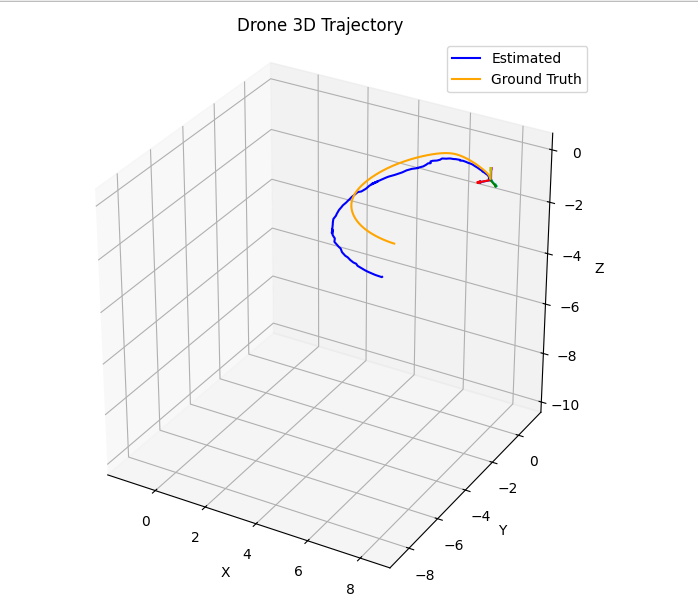
\includegraphics[width=0.8\linewidth]{figures/ekf_results.png}
    \caption{Kalman filter results with tracks from both estimated and ground truth performance.}
    \label{fig:kalman_results}
\end{figure}

It is observed that although the ground truth is tracked by the filter, there is observed drift, particularly on the z-axis. The Kalman Filter was tuned using the process and measurement noise matrices, which were iterated upon with different values to find the best fit. Ultimately, the filter was tuned to get an RMSE of [6.67, 5.41, 1.06] for the x, y and z axes respectively.

\end{document}